\documentclass[shownotes,11pt, aspectratio=169]{beamer}

\usepackage{amsbsy, amsfonts, amsmath, amssymb, appendixnumberbeamer, array, bbm, booktabs, caption, 
            changepage, color, dcolumn, epsfig, etoolbox, eucal, graphics, graphicx, helvet, hyperref, 
            lipsum, longtable, mathpazo, mathrsfs, mathtools, multimedia, multirow, pgfpages, psfrag, rotating, 
            tabularx, tabulary, tfrupee, threeparttable, tikz, url, verbatim}
% These slides also contain speaker notes. You can print just the slides,
% just the notes, or both, depending on the setting below. Comment out the want
% you want.
\setbeameroption{hide notes} % Only slide
%\setbeameroption{show only notes} % Only notes
%\setbeameroption{show notes on second screen=right} % Both
\AtBeginSection[]{
  \begin{frame}
  \vfill
  \centering
  \begin{beamercolorbox}[sep=8pt,center,shadow=true,rounded=true]{title}
    \usebeamerfont{title}\insertsectionhead\par%
  \end{beamercolorbox}
  \vfill
  \end{frame}
}


\usepackage[default]{Fira Sans}
\setbeamertemplate{note page}{\pagecolor{yellow!5}\insertnote}
\usetikzlibrary{positioning}
\usetikzlibrary{snakes}
\usetikzlibrary{calc}
\usetikzlibrary{arrows}
\usetikzlibrary{decorations.markings}
\usetikzlibrary{shapes.misc}
\usetikzlibrary{matrix,shapes,arrows,fit,tikzmark}
\appto\TPTnoteSettings{\footnotesize}
\newcommand{\overbar}[1]{\mkern 2.5mu\overline{\mkern-2.5mu#1\mkern-2.5mu}\mkern 2.5mu}
%%%%

\newcolumntype{d}[0]{D{.}{.}{5}}

\newcommand{\beginbackup}{
   \newcounter{framenumbervorappendix}
   \setcounter{framenumbervorappendix}{\value{framenumber}}
   \setbeamertemplate{footline}
   {
     \leavevmode%
     \hline
     box{%
       \begin{beamercolorbox}[wd=\paperwidth,ht=2.25ex,dp=1ex,right]{footlinecolor}%
%         \insertframenumber  \hspace*{2ex} 
       \end{beamercolorbox}}%
     \vskip0pt%
   }
 }
\newcommand{\backupend}{
   \addtocounter{framenumbervorappendix}{-\value{framenumber}}
   \addtocounter{framenumber}{\value{framenumbervorappendix}} 
}


%\usepackage{graphicx}
\usepackage[space]{grffile}

% These are my colors -- there are many like them, but these ones are mine.
\definecolor{blue}{RGB}{0,114,178}
\definecolor{red}{RGB}{213,94,0}
\definecolor{yellow}{RGB}{240,228,66}
\definecolor{green}{RGB}{0,158,115}
\definecolor{applegreen}{rgb}{0.55, 0.71, 0.0}
\definecolor{ao(english)}{rgb}{0.0, 0.5, 0.0}

\hypersetup{
  colorlinks=false,
  bookmarks=true,
  linkbordercolor = {white},
  linkcolor = {blue}
}


%% I use a beige off white for my background
\definecolor{MyBackground}{RGB}{255,253,218}

%% Uncomment this if you want to change the background color to something else
\setbeamercolor{background canvas}{bg=MyBackground}

%% Change the bg color to adjust your transition slide background color!
\newenvironment{transitionframe}{
  \setbeamercolor{background canvas}{bg=yellow}
  \begin{frame}}{
    \end{frame}
}

\setbeamercolor{frametitle}{fg=blue}
\setbeamercolor{title}{fg=black}
\setbeamertemplate{footline}[frame number]
\setbeamertemplate{navigation symbols}{} 
\setbeamertemplate{itemize items}{-}
\setbeamercolor{itemize item}{fg=blue}
\setbeamercolor{itemize subitem}{fg=blue}
\setbeamercolor{enumerate item}{fg=blue}
\setbeamercolor{enumerate subitem}{fg=blue}
\setbeamercolor{button}{bg=MyBackground,fg=blue,}



% If you like road maps, rather than having clutter at the top, have a roadmap show up at the end of each section 
% (and after your introduction)
% Uncomment this is if you want the roadmap!
% \AtBeginSection[]
% {
%    \begin{frame}
%        \frametitle{Roadmap of Talk}
%        \tableofcontents[currentsection]
%    \end{frame}
% }
\setbeamercolor{section in toc}{fg=blue}
\setbeamercolor{subsection in toc}{fg=red}
\setbeamersize{text margin left=1em,text margin right=1em} 

\newenvironment{wideitemize}{\itemize\addtolength{\itemsep}{10pt}}{\enditemize}

\title[]{\textcolor{blue}{Macroeconomics: The Open Economy}}
\author[SM]{Sumit Mishra}
\institute[IFMR]{\small{\begin{tabular}{c}
IFMR, Sri City \\
\end{tabular}}}

\date{11 November, 2019}

%\documentclass[10pt]{beamer}
%\input{slideclass.tex}







%----------------------------------------------------------------------------------------
%	TITLE PAGE
%----------------------------------------------------------------------------------------


\begin{document}


\begin{frame}
\titlepage % Print the title page as the first slide
\end{frame}
%\colorlinks=true
%\begin{frame}
%\frametitle{Overview} % Table of contents slide, comment this block out to remove it
%\tableofcontents % Throughout your presentation, if you choose to use \section{} and \subsection{} commands, these will automatically be printed on this slide as an overview of your presentation
%\end{frame}

%----------------------------------------------------------------------------------------
%	PRESENTATION SLIDES
%----------------------------------------------------------------------------------------

\section{Chapter 18}
\begin{frame}
\begin{center}
%\begin{figure}[ht]
\centering
 \makebox[\linewidth][c]{
  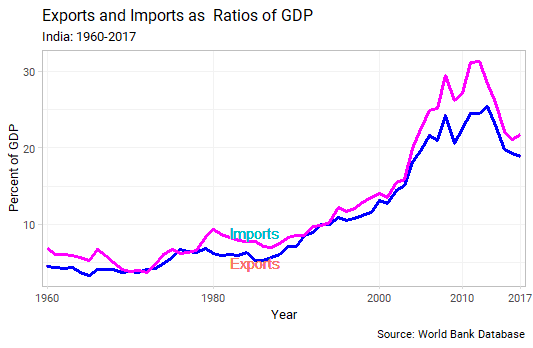
\includegraphics[scale = 0.9]{graphs/L10F01.png}}
%\caption*{Welcome to \textcolor{ao(english)}{impact evaluation methods for business decisions}}
%\end{figure}
\end{center}
\end{frame}

\begin{frame}{Nominal \& Real Exchange Rates}
\begin{itemize}
\item \textbf{Nominal Exchange Rate}: Price of domestic currency in terms of foreign currency. ($E$)
       \begin{itemize}
       \item \textbf{Appreciation}: Increase in the value of the domestic currency.
       \item \textbf{Depreciation}: Fall in the value of the domestic currency.
       \end{itemize}
\vspace{3mm}
\item \textbf{Real Exchange Rate}: Adjust the nominal exchange rate by the relative price levels.
           \[ \epsilon = \frac{EP}{P^{\ast}} \]
        \begin{itemize}
        \item $P$ is the price index in the local economy.
        \item $P^{\ast}$ is the price index for the foreign country.
        \end{itemize}
\end{itemize}
\end{frame}

\begin{frame}{The Balance of Payments}
\textcolor{ao(english)}{Trade Flows} + \textcolor{red}{Financial Flows}

\vspace{6mm}
\pause

\begin{itemize}
\item \textbf{Current Account}:
      \begin{itemize}
      \item Exports and imports.
      \item Net transfers received.
      \end{itemize}
\item \textbf{Capital Account}: Difference between foreign holdings of domestic assets and domestic holdings of foreign assets.
\end{itemize}
\end{frame}

\begin{frame}{The Choice between Domestic and Foreign Assets}
\begin{itemize}
\item Let's say that you have the choice between Indian and Turkish bonds.
     \begin{itemize}
     \item Suppose that you choose Indian bond.
     \item Let $i_t$ be the nominal one-year interest rate. You will get \rupee $(1 + i_t)$ next year.
     \pause
     \item Suppose you choose the Turkish bond.
     \item You must purchase Turkish lira. Let exchange rate be $E_t$.
     \item Let $i_t^{\ast}$ be the interest rate on the Turkish bond. You will get: $E_t\times(1 + i_t^{\ast})$.
     \item Convert this into \rupee: $E_t\times(1 + i_t^{\ast})\times(1/E^{e}_{t+1})$
     \end{itemize}
\pause
\item The choice depends upon:
       \begin{itemize}
       \item[1] Difference between interest rates.
       \item[2] Expected nominal exchange rate in future.
       \item[3] Nominal exchange rate today.
       \end{itemize}
\end{itemize}
\end{frame}

\begin{frame}{Uncovered Interest Parity}
Recall our discussions on choosing between bonds. We assumed that people just care about the expected rate of returns. 
Therefore, the following relation must hold:
 \[ (1 + i_t) = E_t\times(1 + i_t^{\ast})\times\Bigg(\frac{1}{E^{e}_{t+1}}\Bigg) \]
\pause
\vspace{3mm}

This ignores:
\begin{itemize}
\item Transaction costs involved. 
\item Cross-country differential in risk.
\end{itemize}
\end{frame}

\begin{frame}{Interest Rates and Exchange Rates}
We can rewrite 
\[ (1 + i_t) = E_t\times(1 + i_t^{\ast})\times\Bigg(\frac{1}{E^{e}_{t+1}}\Bigg) \]
as
\[ (1 + i_t) = \frac{(1 + i_t^{\ast})}{[1 + (E^{e}_{t+1} - E_t)/E_t]} \]
\pause
Some magic trick later..
\[ i_t \approx i_t^{\ast} - \frac{E^{e}_{t+1} - E_t}{E_t} \]
\pause
\vspace{3mm}

\textit{The domestic interest rate must be equal to the foreign interest rate minus the expected appreciation rate of the domestic currency}.
\end{frame}

\begin{frame}{Example}
\textcolor{red}{Buying Brazilian Bonds}
\begin{itemize}
\item Monthly interest rate on Brazilian bond = 36\%
\item Monthly interest rate on U.S. bonds = 0.2\%
\item Shouldn't investor just run to purchase Brazilian bonds?
\pause
\item The rate of appreciation of Brazilian currency = 34.6\%
\pause
\item The expected returns look much more modest now (1.6\% per month).
\end{itemize}
\end{frame}

\section{Chapter 19}
\begin{frame}{The $IS$ Relation in the Open Economy}
\begin{itemize}
\item The demand for domestic goods:
      \[ Z \equiv C + I + G - IM/\epsilon + X  \]
\item The determinants of $C, I, G$: 
    \begin{itemize}
    \item There shouldn't be any sizeable impact of $\epsilon$ on any of these variables.
    \item There is no direct (or obvious) link between these variables ($C$ and $E$ or $\epsilon$). 
    \end{itemize}
\end{itemize}
\begin{columns}[T] % align columns
\begin{column}{.46\textwidth}
$IM = IM(Y, \epsilon)$
\begin{itemize}
\item $\uparrow Y \Rightarrow \uparrow IM$
\item $\uparrow \epsilon \Rightarrow \uparrow IM$
\end{itemize}
\end{column}
\hfill
\pause
\begin{column}{.44\textwidth}
$X = X(Y^{\ast}, \epsilon)$ [$Y^{\ast}$: Foreign Income]
\begin{itemize}
\item $\uparrow Y^{\ast} \Rightarrow \uparrow X$
\item $\uparrow \epsilon \Rightarrow \downarrow X$
\end{itemize}
\end{column}
\end{columns}
\end{frame}

\begin{frame}{Putting the Components Together}
\makebox[\linewidth][c]{
  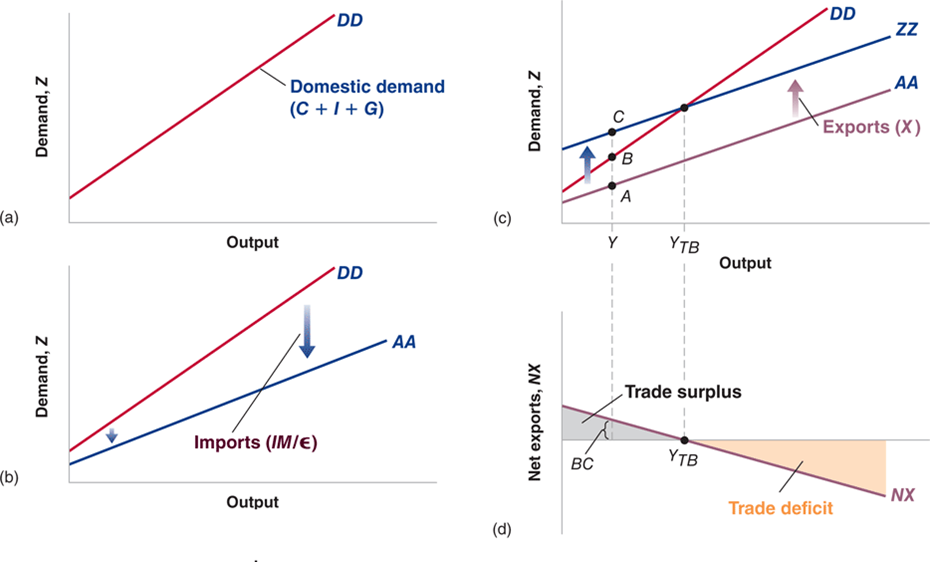
\includegraphics[scale=0.6]{graphs/L10F02.png}}
\end{frame}

\begin{frame}{Equilibrium Output and the Trade Balance}
\begin{columns}[T] % align columns
\begin{column}{.36\textwidth}
\begin{itemize}
\item Domestic output must match the demand
     \[ Y \equiv Z \]
\item Using the components of demand, we get 
     \[ Y = C + I + G + X(Y^{\ast},\epsilon) - IM(Y, \epsilon) \]
\end{itemize}
\end{column}
\hfill
\pause
\begin{column}{.54\textwidth}
\makebox[\linewidth][c]{
  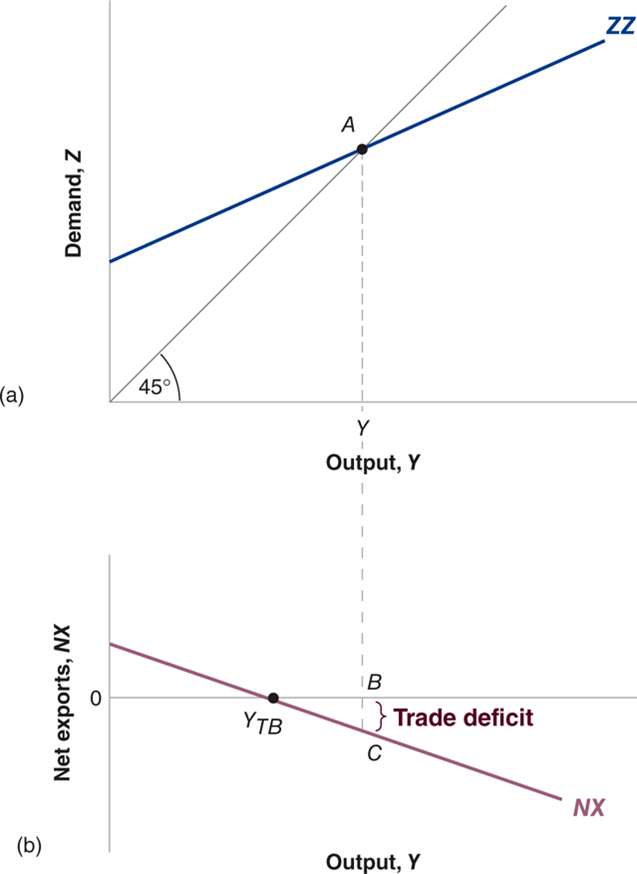
\includegraphics[scale=0.5]{graphs/L10F03.png}}
\end{column}
\end{columns}
\end{frame}

\begin{frame}{Increase in Domestic Demand}
\begin{columns}[T] % align columns
\begin{column}{.36\textwidth}
\begin{itemize}
\item Rise in domestic demand pushes imports up. [Remember: $IM = IM(Y, \epsilon)$]
\item The effect of government spending on output is smaller than it would be in a closed economy. Why? \pause
      \begin{itemize}
      \item Because the demand relation is flatter than demand relation in the closed economy.
      \end{itemize}
\item No impact on exports. \pause Net impact: Trade deficit.
\end{itemize}
\end{column}
\hfill
\pause
\begin{column}{.54\textwidth}
\makebox[\linewidth][c]{
  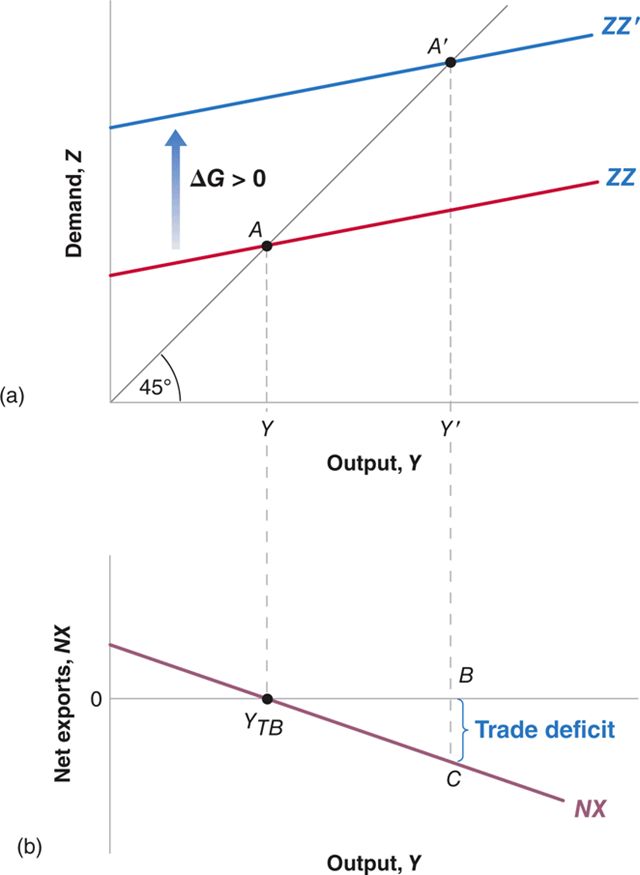
\includegraphics[scale=0.5]{graphs/L10F04.png}}
\end{column}
\end{columns}
\end{frame}

\begin{frame}{Increase in Foreign Demand}
Let there be a rise in foreign output ($\uparrow Y^{\ast}$).
\begin{columns}[T] % align columns
\begin{column}{.36\textwidth}
\begin{itemize}
\item Rise in foreign demand pushes exports up. [Remember: $X = X(Y^{\ast}, \epsilon)$]
\item The demand for domestic goods also moves up.
\item Because domestic demand is up, imports may also increase (but not enough to offset rise in exports).
\end{itemize}
\end{column}
\hfill
\pause
\begin{column}{.54\textwidth}
\makebox[\linewidth][c]{
  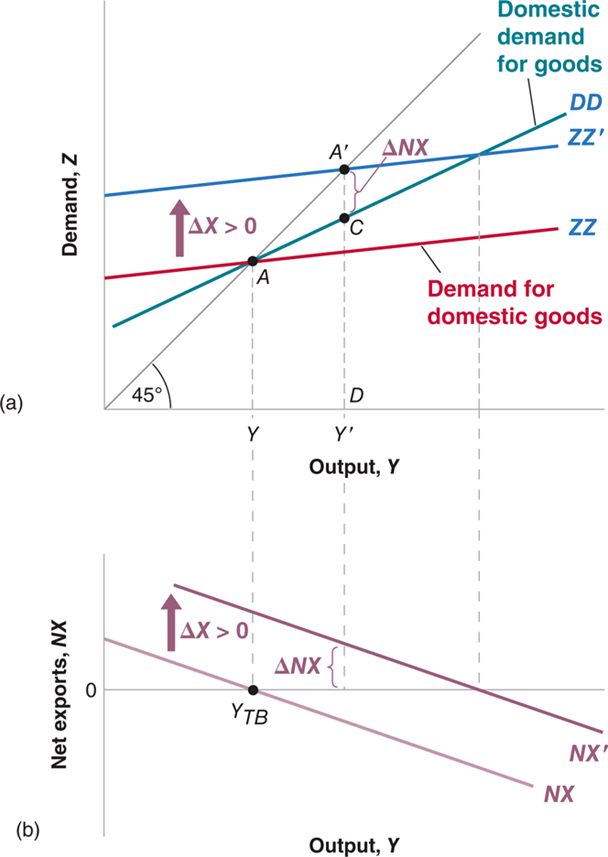
\includegraphics[scale=0.5]{graphs/L10F05.png}}
\end{column}
\end{columns}
\end{frame}

\begin{frame}{Summary: Fiscal Policy}
\vspace{4mm}

\begin{itemize}
\item Changes in domestic fiscal policy: 
     \begin{itemize} 
     \item[1] $\uparrow$ Domestic Demand $\Rightarrow$ $\uparrow$ Domestic Output.
     \item[2] $\uparrow$ Domestic Demand $\Rightarrow$ $\downarrow$ Trade Balance.
     \end{itemize}
\pause
\vspace{4mm}

\item Shifts in foreign fiscal policy: 
      \begin{itemize}
      \item[1] $\uparrow$ Foreign Demand $\Rightarrow$ $\uparrow$ Domestic Output.
      \item[2] $\uparrow$ Foreign Demand $\Rightarrow$ $\uparrow$ Trade Balance.
      \end{itemize}
\end{itemize}
\end{frame}

\begin{frame}{The Marshall Lerner Condition}
\[ NX = X(Y^{\ast}, \epsilon) - IM(Y, \epsilon) \]
Real depreciation affects trade balance through:
    \begin{itemize}
    \item[1] Exports rise.
    \item[2] Imports fall.
    \item[3] The relative price of foreign good in terms of domestic good $1/\epsilon$ increases.
    \end{itemize}
\end{frame}

\begin{frame}{Fiscal Policy + Exchange Rate Policy}
Suppose that economy is running trade deficit, and the government wants to reduce the trade deficit without tinkering with the output.
\begin{itemize}
\item Step 1- Achieve a depreciation such that the net exports increase.
\item Step 2- Reduce government spending to offset the rise in demand due to rising exports.
\end{itemize}
\textcolor{red}{Depreciation + Fiscal Contraction} worked. 
\end{frame}

\begin{frame}
\centering
\makebox[\linewidth][c]{
  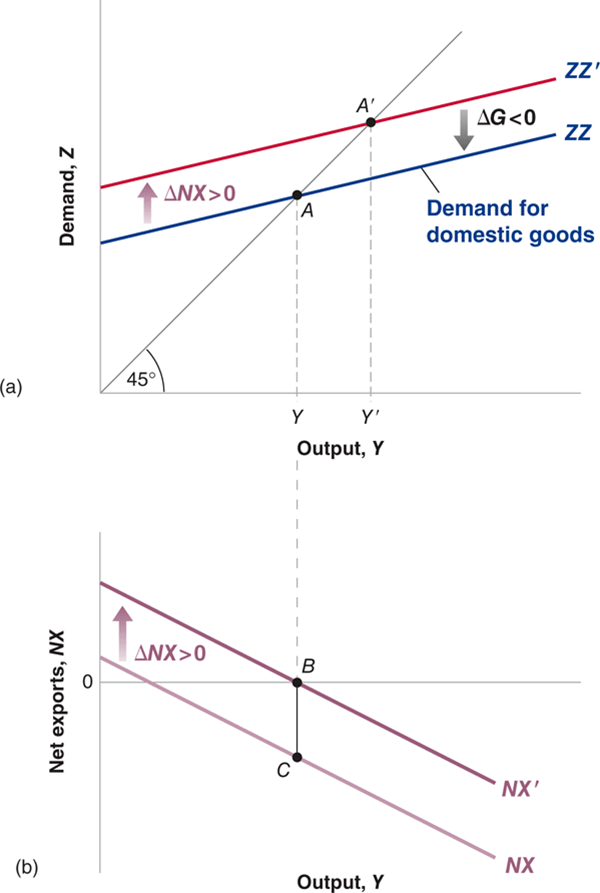
\includegraphics[scale=0.5]{graphs/L10F06.png}}
\end{frame}

\begin{frame}{Savings, Investments, and the Current Account Balance}
Let's try to see how savings-investment relationship can change when you open up the economy.

\begin{itemize}
\item Equilibrium condition: $ Y = C + I + G + NX$ \pause \\ where $ NX = X - IM/\epsilon$.
\pause
\item \[ Y - T - C = I + (G - T) + NX \]
\item Let's add two new terms for- net income from abroad ($NI$) and net transfers from abroad ($NT$).
     \[ (Y + NI + NT - T) - C = I + (G - T) + (NX + NI + NT) \]
\pause
\item \[ \underbrace{(Y + NI + NT - T)}_{\textcolor{red}{\text{Disposable Income}}} - C =  I + (G - T) + \overbrace{(NX + NI + NT)}^{\textcolor{ao(english)}{\text{Current Account}}} \]

\pause
\item $CA = S + (T - G) - I $.
\end{itemize}
\end{frame}

\section{Chapter 20}
\begin{frame}{Equilibrium in the Good Market}
\[ Y = C(Y - T) + I(Y,r) + G - X(Y^{\ast}, \epsilon) + IM(Y, \epsilon) \]
We can rewrite the last term in the equation as $NX(Y,Y^{\ast}, \epsilon)$.
\begin{itemize}
\item $\uparrow r \Rightarrow \downarrow I \Rightarrow \downarrow \text{demand for domestic goods}$
\item $\uparrow \epsilon \Rightarrow \uparrow \text{demand for foreign goods} \Rightarrow \downarrow NX \Rightarrow \downarrow Y$.
\end{itemize}
Let's do away with the distinction between the real and the nominal exchange rate (for now).
\end{frame}

\begin{frame}{Equilibrium in the Financial Market}
\begin{itemize}
\item Money demand is not a function of exchange rate movements. 
\item So, our good old equation hold true here as well
      \[ \frac{M}{P} = YL(i) \]
\end{itemize}
\end{frame}

\begin{frame}{Domestic versus Foreign Bond}
\begin{itemize}
\item The arbitrage condition (the interest parity condition) must hold
     \[ (1 + i_t) = (1 + i_t^{\ast})\Bigg(\frac{E_t}{E_{t+1}^e}\Bigg) \]
\item Let's reorganize this equation in terms of exchange rate.
      \[ E_t = \Bigg(\frac{1 + i_t}{1 + i_t^{\ast}}\Bigg)E_{t+1}^e \]
\item Implications:
      \begin{itemize}
      \item $\uparrow i \Rightarrow \uparrow E_t$
      \item $\uparrow i^{\ast} \Rightarrow \downarrow E_t$
      \item $\uparrow E_{t+1}^e \Rightarrow \uparrow E_t$
       \end{itemize}
\end{itemize}
\end{frame}

\begin{frame}
\begin{columns}[T] % align columns
\begin{column}{.36\textwidth}
 \[ E_t = \Bigg(\frac{1 + i_t}{1 + i_t^{\ast}}\Bigg)E_{t+1}^e \]
 \begin{itemize}
  \item When domestic interest rate = foreign interest rate, $E_t = E_{t+1}^e$.
  \item The higher the domestic interest rate, the higher the exchange rate.
\end{itemize}
\end{column}
\hfill
\pause
\begin{column}{.44\textwidth}
\makebox[\linewidth][c]{
  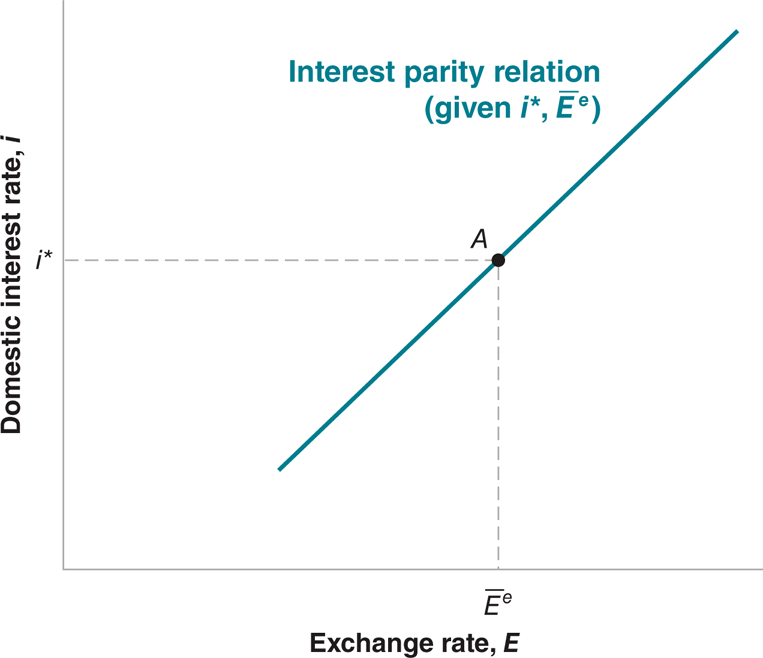
\includegraphics[scale = 0.5]{graphs/L10F09.png}}
\end{column}
\end{columns}
\end{frame}

\begin{frame}{$IS-LM$: Open Economy Version}
\begin{itemize}
\item $IS$ Relation:
     \[ Y = C(Y - T) + I(Y,i) + G + NX(Y,Y^{\ast}, E) \]
\pause
\item $LM$ Relation:
     \[ \frac{M}{P} = YL(i) \]
\pause
\item Interest parity condition:
     \[ E = \Bigg(\frac{1 + i}{1 + i^{\ast}}\Bigg)E^e \]
\end{itemize}
\end{frame}

\begin{frame}{Shifts in the $IS$ Curve}
When domestic interest rate rises:
\begin{itemize}
\item \textcolor{red}{Direct Effect}: $\downarrow I \Rightarrow \downarrow Z \Rightarrow \downarrow Y$.
\item \textcolor{ao(english)}{Indirect Effect} $\uparrow E \Rightarrow \downarrow NX \Rightarrow Z \Rightarrow \downarrow Y$.
\end{itemize}
\end{frame}

\begin{frame}{Fiscal Policy in Open Economy}
$\uparrow$ govt spending $\Rightarrow$...
\begin{itemize}
\item $\uparrow$ Income ($IS$ Curve shifts to the right).
\item $?$ Investment.
\item $\downarrow$ NX
       \begin{itemize}
        \item $\uparrow Y \Rightarrow \uparrow IM$
         \item $\uparrow i \Rightarrow \downarrow X$.
         \end{itemize}
\end{itemize}
\end{frame}

\begin{frame}{Monetary Policy in Open Economy}
%\begin{frame}
Consider the case of increase in money supply. $\Delta M  > 0$.
\begin{itemize}
\item $\downarrow i$ $\Rightarrow$ \pause foreign bonds become attractive.
\item $\downarrow i\Rightarrow$ \pause depreciation.
\item Lower interest rate + depreciation $\Rightarrow \uparrow Y$.
\end{itemize}
\end{frame}

\begin{frame}{Pegging the Exchange Rate}
If the rate is pegged, the future exchange rate will also be expected remain at that value. ($E_t = E_{t+1}^e$)
Therefore,
\[ (1 + i_t) = (1 + i_t^{\ast}) \]
\[\Rightarrow i_t = i^{\ast} \]
Under a fixed exchange, the domestic interest rate must match the foreign interest rate.
\pause
\\
Implication: The $LM$ relation changes.
\[ LM: \frac{M}{P} = YL(i^{\ast}) \]
\end{frame}

\begin{frame}{Trade Policy under Floating Exchange Rate}
Impose tariff/quota such that $\downarrow IM$.
\begin{itemize}
\item $\uparrow NX \Rightarrow \pause \uparrow Y$
\pause
\item $\uparrow Y \Rightarrow \pause \uparrow i$
\pause
\item $\uparrow i \Rightarrow \pause \uparrow E$
\pause
\item Appreciation $\Rightarrow \downarrow X$
\end{itemize}
Net effect of trade policy: $\Delta Y = 0$.
\end{frame}

\begin{frame}{Monetary Policy Under Fixed Exchange Rate}
\begin{itemize}
\item Suppose because of increasing output, money demand goes up.
\item The equilibrium interest rate increases.
\item $i > i^{\ast}$.
\item The currency might appreciate. 
\item To pull the interest rate down, \pause the central bank must increase the money supply.
\end{itemize}
\textbf{Bottomline:} Under fixed exchange rate, the central bank gives up monetary policy as a policy instrument. 
\end{frame}

\begin{frame}{Fiscal Policy Under Fixed Exchange Rate}
Reduce $T$.
\begin{itemize}
\item $IS$ curve moves to the right.
\item $i > i^{\ast}$.
\item The $LM$ curve must move downwards. (Why?)
\item Net effect: $\uparrow Y$.
\end{itemize}
\end{frame}

\begin{frame}{Trade Policy under Fixed Exchange Rate}
Impose tariff/quota such that $\downarrow IM$.
\begin{itemize}
\item $\uparrow NX \Rightarrow \pause \uparrow Y$
\pause
\item $\uparrow Y \Rightarrow \pause \uparrow i$
\pause
\item $\uparrow i \Rightarrow $ \pause LM Curve must shift to the right.
%\pause
%\item Appreciation $\Rightarrow \downarrow X$
\end{itemize}
Net effect of trade policy: $\Delta Y > 0$.
\end{frame}


\begin{frame}
\frametitle{The Mundell-Fleming Model: Summary of Policy Effects}
\linespread{1}
\begin{table}[htbp]
  \centering
  %\caption*{The Mundell-Fleming Model: Summary of Policy Effects}
  \begin{threeparttable}
    %\centering
    \begin{tabular}{lccccccc}
          & \multicolumn{7}{c}{Exchange Rate Regime} \\
\cmidrule{2-8}          & \multicolumn{3}{c}{Floating} &       & \multicolumn{3}{c}{Fixed} \\
\cmidrule{2-4}\cmidrule{6-8}          & \multicolumn{7}{c}{Impact On} \\
\cmidrule{2-8}    \multicolumn{1}{l}{Policy} & \multicolumn{1}{l}{$Y$} & \multicolumn{1}{l}{$E$} & \multicolumn{1}{l}{$NX$} &       & \multicolumn{1}{l}{$Y$} & \multicolumn{1}{l}{$E$} & \multicolumn{1}{l}{$NX$} \\
    \midrule
    Fiscal Expansion & 0     & $\uparrow$   & $\downarrow$    &       & $\uparrow$     & 0     & 0 \\
    Monetary Expansion & $\uparrow$   & $\downarrow$     & $\uparrow$     &       & 0     & 0     & 0 \\
    Import Restrictions & 0     & $\uparrow$     & 0     &       & $\uparrow$    & 0     & $\uparrow$ \\
    \bottomrule
    \end{tabular}%
    \begin{tablenotes}
    \tiny
\item This table shows the direction of impact of various economic policies on income $Y$, the
exchange rate $e$, and the trade balance $NX$. A ``$\uparrow$'' indicates that the variable increases; a ``$\downarrow$''
indicates that it decreases; a ``0'' indicates no effect. Remember that the exchange rate is
defined as the amount of foreign currency per unit of domestic currency (for example, 100 EUR per INR).
        \end{tablenotes}
     \end{threeparttable}
  %\label{tab:addlabel}%
\end{table}%
\end{frame}

\section{Chapter 21}

\begin{frame}{Agenda}
\begin{itemize}
\item Open economy in the medium run.
\item Fixed Exchange Rates and Crises.
\item Flexible Exchange Rates and Problems.
\item Material: Chapter 21, Blanchard.
\end{itemize}
\end{frame}

\begin{frame}{The Nominal and The Real Exchange Rate}
\[ \epsilon = E\times\frac{P}{P^{\ast}} \]
Real exchange rate adjustment can happen via:
\begin{itemize}
\item The domestic price level change ($P$).
\item The foreign price level change ($P^{\ast}$).
\end{itemize}
\end{frame}

\begin{frame}{The $AS-AD$ Model Under Fixed Exchange Rate}
\begin{equation*}
AD: Y = Y(\epsilon, G, T)
\end{equation*}
Note that $M/P$ is missing. (Why?)
\pause
\begin{equation*}
AS: P = P^e(1 + m)F\Bigg(1 - \frac{Y}{L}, z\Bigg)
\end{equation*}
\end{frame}

\begin{frame}{Equilibrium with Fixed Exchange Rate}
\begin{itemize}
\item $\uparrow P \Rightarrow \uparrow \epsilon $.
\item $\uparrow \epsilon \Rightarrow \downarrow \text{demand for domestic goods}$.
\end{itemize}
Let $Y < Y_n$. What happens in the medium run?
\begin{itemize}
\item The $AS$ curve keeps moving downwards until $Y = Y_n$. (Old Channel)
\item In this process, $\downarrow P$.
\item $\downarrow P \Rightarrow \downarrow \epsilon$. (New Channel)
\item The output keeps increasing until $Y = Y_n$.
\end{itemize}
\end{frame}

\begin{frame}
 \makebox[\linewidth][c]{
  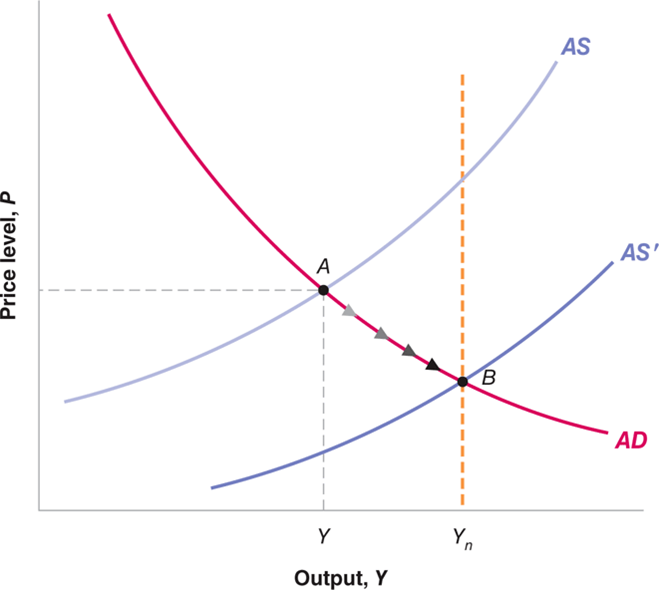
\includegraphics[scale = 0.55]{graphs/L10F14.png}}
\end{frame}

\begin{frame}{Whither Devaluation?}
\begin{columns}[T] % align columns
\begin{column}{.4\textwidth}
\begin{itemize}
\item Instead of letting the prices dictate the process of adjustment, why not devalue?
     \begin{itemize}
     \item Exports become attractive.
     \item $AD$ curve moves to the right. 
     \pause
     \item The trouble: \textcolor{red}{$\uparrow$ Inflation}
     \end{itemize}
\end{itemize}
\end{column}
\hfill
\pause
\begin{column}{.54\textwidth}
\makebox[\linewidth][c]{
  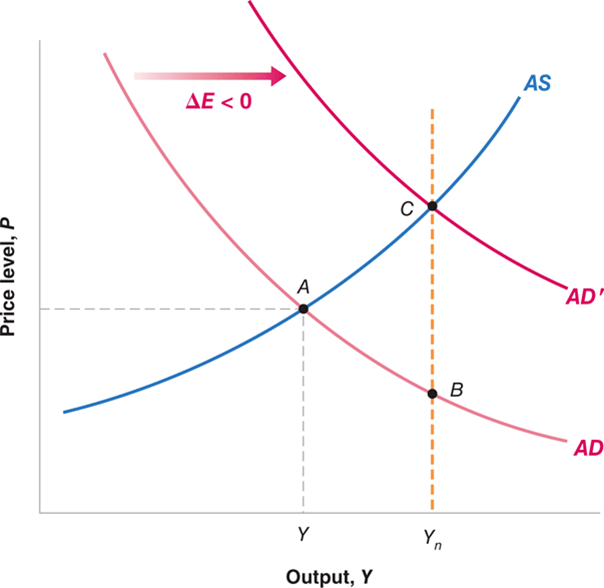
\includegraphics[scale = 0.55]{graphs/L10F15.png}}
\end{column}
\end{columns}
\end{frame}


\begin{frame}{Exchange Rate Crises under Fixed Exchange Rate}
\begin{itemize}
\item The real exchange rate may be too high. (Diagnosis: depreciation)
\item Since interest rates are fixed to foreign levels, the country may be forced to devalue the currency.
\end{itemize}
What choices does the govt have?
\begin{itemize}
\item Devalue.
\item Be prepared for very high interest rates.
\end{itemize}
\end{frame}

\begin{frame}{Flexible Exchange Rate System: Problems}
Current exchange rate depends on two sets of factors:
\begin{itemize}
 \item Current and expected future domestic and foreign interest rates.
 \item The expected future exchange rate.
\end{itemize}
\pause
When the Bretton Woods era was over, everyone thought that the flexible exchange rate would be stable.
\begin{itemize}
\item It was only in the mid-1970s that economists understood what we just learnt. 
\item Because the current exchange rate depends so much upon the future, \pause economies with flexible exchange rate system should be prepared for huge fluctuations in the exchange rate.
\end{itemize}
\end{frame}


\end{document}
